 \documentclass{report}
 
\usepackage[utf8]{inputenc} 
\usepackage[T1]{fontenc}      
\usepackage[top=2.0cm, bottom=3cm, left=3.0cm, right=3.0cm]{geometry}
\usepackage{graphicx}
\usepackage{wrapfig}
\usepackage{amsmath,esint }
\usepackage{amssymb}
\graphicspath{{figures/}{../figures}}

\newcommand*\dif{\mathop{}\!\mathrm{d}}
\newcommand*\diver{\mathop{}\!\mathrm{div}}
\newcommand*\grad{\mathop{}\!\mathrm{grad}}

\begin{document}

\section*{Force exercée sur un barrage $\bullet\circ\circ$}

On considère un barrage de lac rempli d'une hauteur d'eau $H$. La forme de sa paroi en contact avec l'eau est décrite par l'équation $z=kx^2$, comme indiqué sur le schéma ci-dessous. Le barrage a une longueur $L$ selon $y$.

\begin{center}
	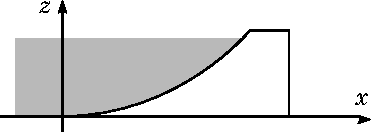
\includegraphics[scale=1]{barrage.pdf}
\end{center}

\begin{itemize}

	\item[$\diamond$] A partir d'un bilan de force, démontrer la relation fondamentale de la statique des fluides dans l'eau : 
	\begin{align*}
		\vec{\grad}(P) - \rho\vec{g}=\vec{0}
	\end{align*}
		où $\rho$ est la densité massique de l'eau, supposée constante et $\vec{g}$ le champ de pesanteur terrestre.
		
		\item[$\diamond$] Donner l'expression du champ de pression $p$ dans l'eau.
		
		\item[$\diamond$] Déterminer les forces horizontales et verticales exercées par le lac sur le barrage.

\end{itemize}

\newpage

\section*{\textit{Correction - Force exercée sur un barrage}}

\begin{itemize}

	\item[$\diamond$] Il s'agit de la démonstration classique de l'équation de statique des fluides. Le bilan des forces (pression et gravité) sur un volume élémentaire $\dif V=\dif x \dif y \dif z$ d'air situé au point $M=(x,y,z)$ s'écrit
	\begin{align*}
		-P(x,y,z+ \dif z)\dif x\dif y\vec{e}_z+P(x,y,z)\dif x\dif y\vec{e}_z+\rho\vec{g}=\vec{0}
	\end{align*}
	On omis les variations de pression selon $x$ et selon $y$ mais qui sont traitées de la même manière qu'en $z$. On trouve alors rapidement l'expression $\vec{\grad}(P) + \rho\vec{g}=\vec{0}$ avec le développement de Taylor de $P(z+dz)$.
	
	\item[$\diamond$] En utilisant la relation précédente : 
	
	\begin{align*}
		p(z) = p_0+\rho g (H-z)
	\end{align*}
		
		\item[$\diamond$] Il faut faire un bilan des forces, en "zoomant" sur la paroi du barrage en un point $(x,z)$ de la surface. La force élémentaire créée par la pression est $d\vec{F}=p(x)dS\vec{n}$, où $\vec{n}$ est la normale à la surface : $\vec{n}=\sin\alpha\vec{e}_x-\cos\alpha\vec{e}_z$, en notant $\alpha$ l'angle la pente du barrage en ce point, cad $\tan\alpha=dz/dx$.
		
		Pour la force horizontale, selon $\vec{e_x}$ :
		
	\begin{align*}
		dF_x = p(z)\sqrt{dx^2+dz^2}L\sin\alpha=p(z)Ldz
	\end{align*}
	car $dS = Ldl=\sqrt{dx^2+dz^2}L$ et $\sin\alpha=dz/dl$. On a donc :
	\begin{align*}
		F_x = \int_0^H p(z)Ldz=\left[ p_0+\frac{\rho g H}{2}\right] LH
	\end{align*}
	
		Pour la force verticale, selon $\vec{e_z}$ :
		
	\begin{align*}
		dF_z= p(z)\sqrt{dx^2+dz^2}L\cos\alpha = -p(z)Ldx
	\end{align*}
	car $\cos\alpha=dx/dl$. En posant $x_0$ tel que $H=kx_0^2$, on a donc :
	\begin{align*}
		F_z = \int_0^{x_0} p(z)Ldz=L\int_0^{x_0} (p_0+\rho g (H-kx^2)dz=-Lx_0p_0-\frac{2}{3}L\rho g x_0H
	\end{align*}

\end{itemize}

\newpage

\section*{Pression dans une étoile $\bullet\bullet\circ$}

Soit une étoile sphérique de rayon $R$ et de masse $M$, constituée de gaz. On note respectivement $p(r)$, $\rho(r)$ et $\vec{g}(r)$ la pression, la densité et le champ de gravitation dans l'étoile à une distance $r$ du centre. On souhaite connaître ces quantités au sein de l'étoile. 

\begin{itemize}

	\item[$\spadesuit$] On admet que le champ de gravitation et la densité sont reliés par la relation :
	\begin{align*}
		\mathbf{div}\vec{g}(r)=-4\pi G\rho(r)
	\end{align*}
où $\rho$ est la constante gravitationnelle. 
Déterminer $g(r)$ en fonction d'une intégrale de $\rho$ que l'on déterminera.

	\item[$\spadesuit$] A partir d'un bilan de force, démontrer la relation fondamentale de la statique des fluides dans le gaz de l'étoile : 
	\begin{align*}
		\vec{\grad}(p) - \rho\vec{g}=\vec{0}
	\end{align*}
	
	\item[$\spadesuit$] Dans le cas où la masse volumique est une constante, cad $\rho(r)=\rho_0$, déterminer le champ de gravité $\vec{g}(r)$ et le champ de pression $p(r)$.
	
	\item[$\spadesuit$] On suppose maintenant que le gaz se comprime au fur et à mesure que la pression augmente au sein de l'étoile, en suivant la loi suivante : 
	\begin{align*}
		\frac{P}{\rho^2}= C
	\end{align*}
	où $C$ est une constante quelconque. 
	
	Trouver une équation différentielle en $\rho(r)$ et la résoudre en introduisant la fonction $f(r)=r\rho(r)$.

\end{itemize}

\newpage

\section*{\textit{Corrige - Pression dans une étoile}}

\section*{Pression dans une étoile $\bullet\bullet\circ$}

\begin{itemize}

	\item[$\spadesuit$] En utilisant le théorèeme de Green-Ostravaski, sur une sphère de rayon $r$ :
	\begin{align*}
		g(r)=-\frac{4\pi G}{r^2}\int_0^r dr' r'^2 \rho(r')
	\end{align*}

	\item[$\spadesuit$] Le classique, cf les corrections précédentes.
	
	\item[$\spadesuit$] On utilise l'expression intégrale précédente :
	\begin{align*}
		g(r)=-\frac{M_eG}{R^3}r
	\end{align*}
	avec $M_e$ la masse de l'étoile. 
	
	\item[$\spadesuit$] On suppose maintenant que le gaz se comprime au fur et à mesure que la pression augmente au sein de l'étoile, en suivant la loi suivante : 
	\begin{align*}
		\frac{P}{\rho^2}= C
	\end{align*}
	où $C$ est une constante quelconque. 
	
	Trouver une équation différentielle en $\rho(r)$ et la résoudre en introduisant la fonction $f(r)=r\rho(r)$.

\end{itemize}

\newpage

\section*{Structure de l'atmosphère $\bullet\bullet\bullet$}

La troposphère constitue la partie basse de l'atmophère dans laquelle nous vivons, du niveau de la mer jusqu'à une altitude comprise entre 8 et 15km. On peut considérer la troposphère comme un gaz parfait de coefficient thermodynamique $\gamma=7/5$, de masse molaire $M=28.965$g.mol$^{-1}$, soumis à la gravitation terrestre, modélisée par l'accélération de la pesanteur $g=9.81$m.s$^{-2}$ supposée constante avec l'altitude (représentée par la variable $z$). La pression au niveau de la mer $z=0$ est $P_0=10^5$Pa et la température est $T_0=$293K. On souhaite connaître l'évolution de la pression $P$ et de la tempérture $T$ avec l'altitude.

\begin{itemize}

	\item[$\vartriangle$] A partir d'un bilan de force, démontrer la relation fondamentale de la statique des fluides pour l'atmosphère : 
	\begin{align*}
		\vec{\grad}(P) - \rho\vec{g}=\vec{0}
	\end{align*}
		où $\rho$ est la densité massique de l'atmosphère.
		
	\item[$\vartriangle$] Redémontrer dans le cas classique de l'atmopshère isotherme ($T(z)=T_0$) l'expression de la pression $P(z)$ et $\rho(z)$. On mettra en évidence une altitude caractéristique $H$ à déterminer. En quoi ce modèle est-il limité ?
		
	\item[$\vartriangle$] Pour déterminer l'évolution de la pression et de la température avec l'altitude, on suppose qu'un volume $V$ d'air subit une transformation adiabatique réversible (et non plus isotherme) lorsqu'il change d'altitude. Montrer alors que la pression $P$ et la densité $\rho$ de l'air sont alors reliées par :
	\begin{align*}
		\rho = \frac{MP_0}{RT_0}\left(\frac{P}{P_0} \right) ^{1/\gamma}
	\end{align*}

	\item[$\vartriangle$] En déduire l'évolution de la pression avec l'altitude $P(z)$, de la densité $\rho(z)$ puis celle de la température $T(z)$. Commenter en mettant en évidence l'altitude caractéristique $H$ vue précédemment. Dans ce modèle, quelle est alors l'épaisseur de l'atmosphère ?
	
	\item[$\vartriangle$] De combien chute la température lorsqu'on monte à 1000m d'altitude d'après ce modèle ? Quelle est la pression et la densité de l'air au sommet de l'Everest (8848m) ?
	
	\item[$\vartriangle$] En réalité, le gradient de température diminue de $7.7\cdot10^{-3}$K.m$^{-1}$. Cela s'explique par le fait que une transformation thermodynamique dans l'atmosphère (comme évoqué ci-dessus) n'est pas parfaitement adiabatique et que le gaz n'est pas sec. Il peut néanmoins être modélisé par un coefficient thermodynamique $\gamma_{eff}\neq\gamma$. Estimer $\gamma_{eff}$. Commenter. 

\end{itemize}

\newpage

\section*{\textit{Correction - Structure de l'atmosphère}}

\begin{itemize}

	\item[$\vartriangle$] Il s'agit de la démonstration classique de l'équation de statique des fluides. Le bilan des forces (pression et gravité) sur un volume élémentaire $\dif V=\dif x \dif y \dif z$ d'air situé au point $M=(x,y,z)$ s'écrit
	\begin{align*}
		-P(x,y,z+ \dif z)\dif x\dif y\vec{e}_z+P(x,y,z)\dif x\dif y\vec{e}_z+\rho\vec{g}=\vec{0}
	\end{align*}
	On omis les variations de pression selon $x$ et selon $y$ mais qui sont traitées de la même manière qu'en $z$. On trouve alors rapidement l'expression $\vec{\grad}(P) + \rho\vec{g}=\vec{0}$ avec le développement de Taylor de $P(z+dz)$.
	
	\item[$\vartriangle$] Dans l'hypothèse d'une transformation adiabatique réversible, un volume $V$ d'air changeant d'altitude suit la loi de Laplace $PV^\gamma=cste$. Comme la densité $\rho$ du gaz contenu dans ce volume $V$ est inversement proportionnelle à celui-ci, on a :
	\begin{align*}
		\rho = cste\times P^{1/\gamma}
	\end{align*}
	Pour déterminer la constante, on utilise la loi des gaz parfait à l'altitude $z_0$ : $P_0V=nRT_0$, ce qui donne $\rho_0=\frac{MP_0}{RT_0}$. On a donc :
	\begin{align*}
		\rho = \rho_0\left(\frac{P}{P_0} \right) ^{1/\gamma}=\frac{MP_0}{RT_0}\left(\frac{P}{P_0} \right) ^{1/\gamma}
	\end{align*}
	
	\item[$\vartriangle$] Avec l'équation de statique des fluide, on a donc :
	\begin{align*}
		\frac{\dif P}{\dif z}=-\rho g = -\frac{Mg}{RT_0}P_0\left(\frac{P}{P_0} \right) ^{1/\gamma}
	\end{align*}
	On introduit le paramètre $H=\frac{RT_0}{Mg}$ homogène à une altitude et la variable de pression réduite $p=P/P_0$. L'équation différentielle devient alors :
	\begin{align*}
		\frac{\dif p}{\dif z}=-\frac{1}{H}p^{1/\gamma}
	\end{align*}	
	La solution est alors :
	
\noindent\fbox{\parbox{\linewidth\fboxrule\fboxsep}{
	\begin{align*}
		p(z)=\left(1-\frac{\gamma-1}{\gamma}\frac{z}{H} \right)^{\frac{\gamma}{\gamma-1}}
	\end{align*}
	}}
	
	La densité se trouve grâce à la relation explicitée à la question précédente :
	
\noindent\fbox{\parbox{\linewidth\fboxrule\fboxsep}{
	\begin{align*}
		\rho(z)=\frac{P_0}{Hg}\left(1-\frac{\gamma-1}{\gamma}\frac{z}{H} \right)^{\frac{1}{\gamma-1}}
	\end{align*}
	}}	
	
	La température se trouve grâce à la relaiton de Laplace, $T^\gamma P^{1-\gamma}=cste$. On a alors $T=T_0\left( \frac{P}{P_0}\right)^\frac{\gamma-1}{\gamma}=T_0p^\frac{\gamma-1}{\gamma}$, donc :
	 
	 	
\noindent\fbox{\parbox{\linewidth\fboxrule\fboxsep}{
	\begin{align*}
		T(z)=T_0\left(1-\frac{\gamma-1}{\gamma}\frac{z}{H} \right)
	\end{align*}
	}}

Les fonctions $P$, $\rho$ et $T$ ne sont définies si et seulement si $1-\frac{1-\gamma}{\gamma}\frac{z}{H}>0$, cad si $z<\frac{\gamma}{\gamma-1}H\simeq 29.75$km. Il n'y a plus du tout de gaz au-delà !

	\item[$\vartriangle$]  La température décroit linéairement avec l'altitude, c'est un résultat que l'on retrouve expérimentalement : plus on monte, plus il fait froid ! Plus précisément, elle diminue de $T_0\frac{\gamma}{1-\gamma}\frac{1}{H}\simeq9.77\cdot10^{-3}$ $^{\circ}$C pour une élévation de 1m, soit une chute de 9.77$^{\circ}$C pour 1000m. 
	
	Au sommet de l'Everest, la pression est de seulement 1/3 celle au niveau de la mer, et la densité seulement la moitié.
	
\begin{figure}[!h]
	\centering
	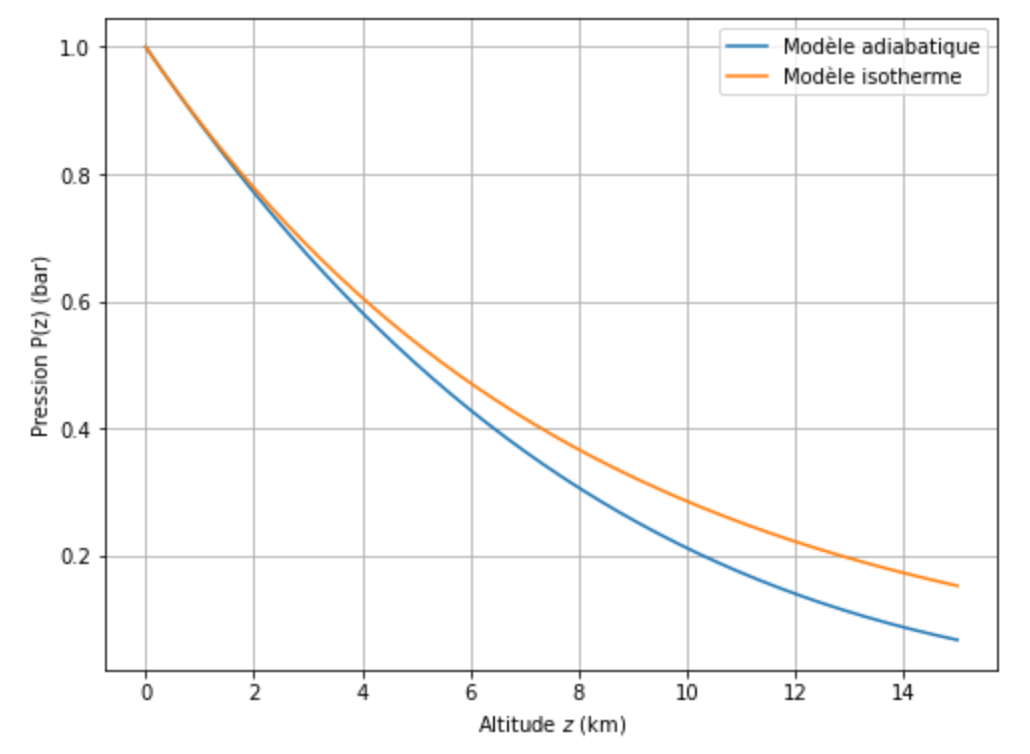
\includegraphics[width=0.5\linewidth]{exo_atmo1.png}
\end{figure}
\begin{figure}[!h]
	\centering
	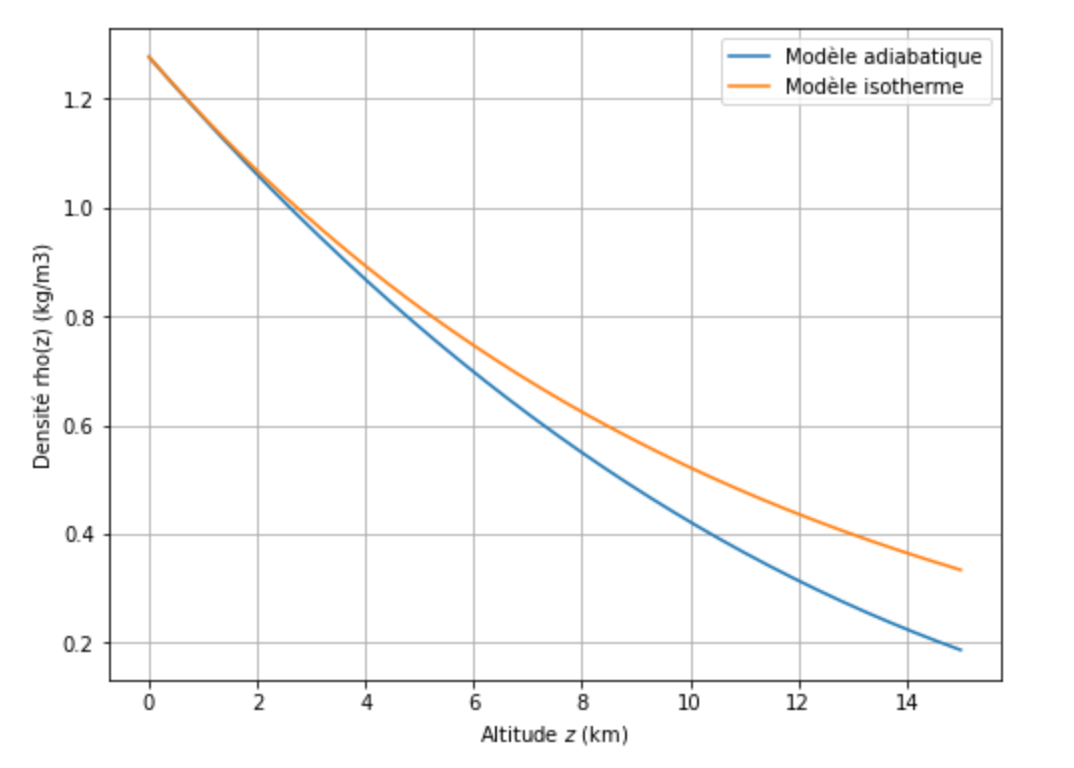
\includegraphics[width=0.5\linewidth]{exo_atmo2.png}
\end{figure}
\begin{figure}[!h]
	\centering
	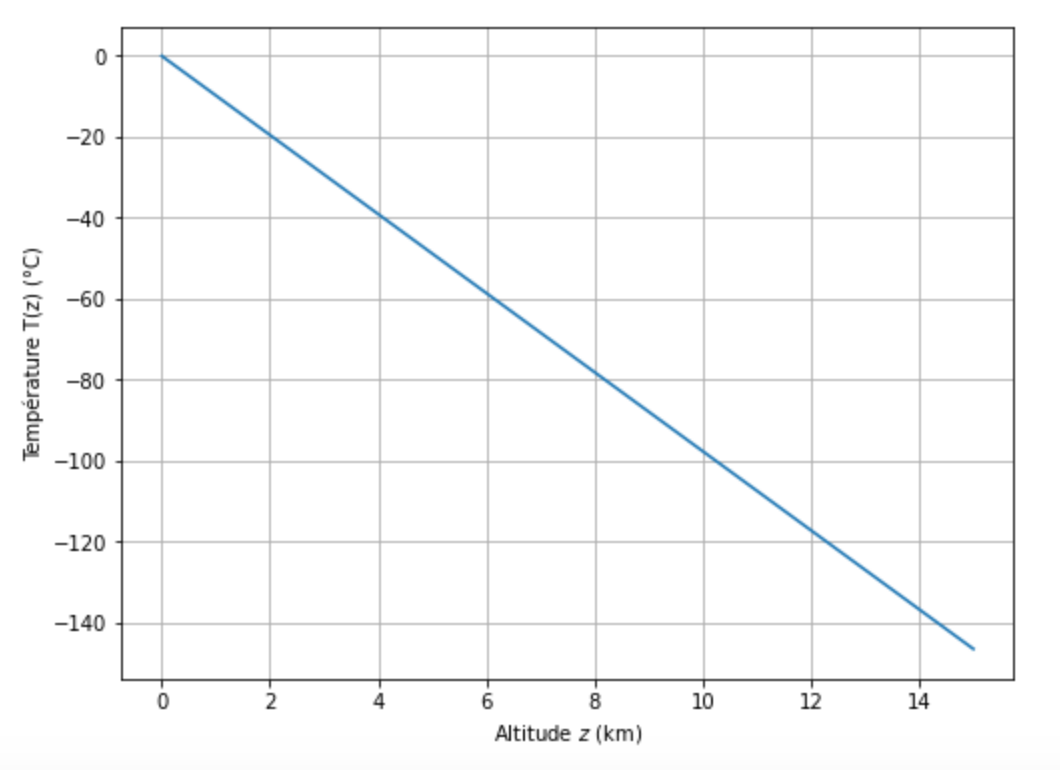
\includegraphics[width=0.5\linewidth]{exo_atmo3.png}
\end{figure}

	\item[$\vartriangle$] L'atmosphère réelle permet des échanges thermiques même faibles. Le gradient de température est un peu plus faible, et coefficient thermodynamique $\gamma_{eff}$ est plus faible, correspondant à une situation où l'on est pas parfaitement adaibatique. Pour le retrouver, on utilise le gradient de température :
	\begin{align*}
		\frac{\dif T}{\dif z}=-T_0\frac{\gamma-1}{\gamma H}=-Mg\frac{\gamma-1}{\gamma R}
	\end{align*}
Pour $\frac{\dif T}{\dif z}=-7.7\cdot10^{-3}$K.m$^{-1}$, on trouve $\gamma_{eff}=1,26$.

	\item[$\vartriangle$] Le modèle d'atmosphère isotherme correspond au cas où $\gamma_{eff}=1$. En effet, dans ce cas là on retrouve la loi des gaz parfait $PV=cste=nRT$, on voit aussi que l'atmosphère a un graident de température nulle et une extension infinie : $z<\frac{\gamma}{\gamma-1}H\longrightarrow\infty$. D'autre part, les fonctions pécédentes convergent vers la décroissance exponentielles de l'atmosphère isotherme :
	\begin{align*}
		P(z)&=P_0\left(1-\frac{\gamma-1}{\gamma}\frac{z}{H} \right)^{\frac{\gamma}{\gamma-1}}\\
		&=P_0\exp\left(\frac{\gamma}{\gamma-1}\ln\left(1-\frac{\gamma-1}{\gamma}\frac{z}{H} \right)\right) \\
		&\xrightarrow[\gamma\to1]{} P_0\exp\left(-\frac{z}{H} \right) 
	\end{align*}

\end{itemize}

\newpage

\section*{Résultante des forces sur une digue $\bullet\circ\circ$}

Une digue verticale de hauteur totale $H$ et de longueur $5H$ sépare deux bassins remplis d'eau, de hauteurs $h_1=3H/4$ d'un côté et $h_2=H/2$ de l'autre. La pression de l'air atmosphérique est notée $P_0$ (elle est uniforme) et la masse volumique de l'eau est notée $\mu_0$.

Quelle est la résultante des forces de pression sur la digue ?

\newpage

\section*{\textit{Correction - Résultante des forces sur une digue}}

En notant $z$ l'altitude, avec $\vec{g}=-g\vec{e}_z$, le champ de pression est à gauche $P_0+\mu_0g(h_1-z)$ pour $z\in[0,h_1]$ et $P_0$ pour $z\in[h_1, H]$. A droite, $P_0+\mu_0g(h_2-z)$ pour $z\in[0,h_2]$ et $P_0$ pour $z\in[h_2, H]$. La résultante des forces est donc issue de deux forces dans l'air, et de deux forces dans l'eau.
\begin{align*}
	f_{1e}&=\int_{z=0}^{h_1}\int_{y=0}^{5H}(P_0+\mu_0g(h_1-z))dydz \\
	&=5H\left(P_0h_1+\mu_0g\frac{h_1^2}{2} \right) 
\end{align*}
Pour la pression dans l'air :
\begin{align*}
	f_{1a}&=\int_{z=h_1}^{H}\int_{y=0}^{5H}P_0dydz \\
	&=5HP_0(H-h_1)
\end{align*}
Et donc :
\begin{align*}
	f_1=5H\left(P_0H+\mu_0g\frac{h_1^2}{2} \right) 
\end{align*}
De même : 
\begin{align*}
	f_1=-5H\left(P_0H+\mu_0g\frac{h_2^2}{2} \right) 
\end{align*}
Donc la résultante est :
\begin{align*}
	f=5H\frac{\mu_0 g}{2}(h_1^2-h_2^2)=\frac{25\mu_0gH^3}{32}
\end{align*}

\newpage

\end{document}
